\documentclass[twocolumn,a4paper]{jsarticle}
%
\usepackage[dvipdfmx]{graphicx}
\usepackage{amsmath,amssymb}
\usepackage{bm}
\usepackage{ascmac}
%
\setlength{\textwidth}{\fullwidth}
\setlength{\textheight}{40\baselineskip}
\addtolength{\textheight}{\topskip}
\setlength{\voffset}{-0.2in}
\setlength{\topmargin}{0pt}
\setlength{\headheight}{0pt}
\setlength{\headsep}{0pt}
%
\newcommand{\divergence}{\mathrm{div}\,}  %ダイバージェンス
\newcommand{\grad}{\mathrm{grad}\,}  %グラディエント
\newcommand{\rot}{\mathrm{rot}\,}  %ローテーション
%
\title{タイトル}
\author{佐原優衣}
\date{}

\begin{document}
\maketitle

\section{はじめに}

\begin{itemize}
  \item item1
  \item item2
  \item ...
  \item itemN
\end{itemize}

\section{見出し}

\begin{figure}
  \centering
  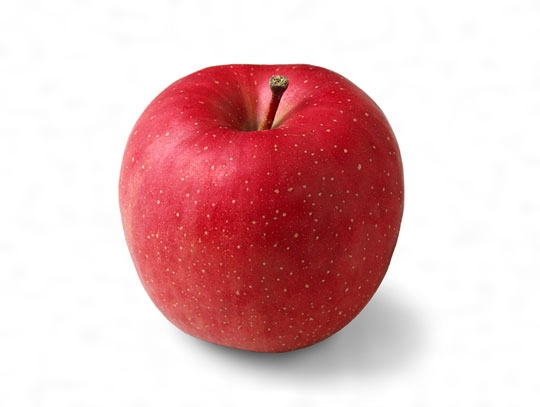
\includegraphics[width=5cm]{apple.jpg}
  \caption{林檎の図}
  \label{app}
\end{figure}

\section{おわりに}
文献\cite{key1}

\begin{thebibliography}{3}
  \bibitem{key1} 参考文献の名前・著者1
  \bibitem{key2} 参考文献の名前・著者2
  \bibitem{keyN} 参考文献の名前・著者N
\end{thebibliography}

\end{document}